\section*{Mutagenesi \emph{in vitro}}

	\subsection*{Introduzione}
        Questo esperimento vuole verificare l'efficacia e la precisione della polimerasi in presenza di sostanze tossiche e/o inibitorie.
	L'organismo modello utilizzato è il lievito \emph{Saccharomyces Cerevisiae} in forma aploide.
	Viene utilizzata come sostanza inibitoria il cloruro di manganese \emph{$MnCl_2$}.
	Il DNA prodotto viene poi visualizzato attraverso \emph{PCR} ed elettroforesi.
        
		\subsubsection*{Polimerase chain reaction \emph{PCR}}
		La \emph{PCR} \`e una tecnica in vitro in cui viene utilizzato il calore per separare le due eliche di DNA.
		In natura questo compito viene svolto da un'elicasi.
       		Un successivo abbassamento della temperatura permette il legame di un primer a una sequenza precisa di DNA.
		Questo permettere alla \emph{PCR} di trovare un \emph{$3'$-OH} da cui iniziare la replicazione.
		Varie ripetizioni del processo permettono di amplificare il DNA.

		\subsubsection*{Effetti del cloruro di manganese}
		Gli ioni magnesio sono usati come catalizzatori della polimerizzazione favorendo la sostituzione nucleofilica del \emph{$3'$-OH} libero del primer con il fosfato del nucleotide.
		Ci si chiede se il manganese sia in grado di competere con il magnesio per l'accesso allosterico e come possa cambiarne l'efficienza.
		Per verificare questo fatto viene svolta una \emph{PCR} in presenza di diverse concentrazioni di cloruro di manganese.

		\subsubsection*{DNA da amplificare}
        	La sequenza di DNA da amplificare codifica per un gene reporter.
		Nella cellula verrà inserito per trasformazione un plasmide linearizzato \emph{pRDI22}.
		Questo plasmide contiene oltre al gene reporter, il gene \emph{leu} un'origine di replicazione e una regione centromerica.
		Il gene \emph{leu} viene inserito in quanto il ceppo di \emph{Saccharomyces cerevisiae} \`e auxotrofo per la leucina.
		Questo permette di selezionare le colonie in cui il plasmide \`e stato trasformato.
		Il ceppo per l'adenina \`e auxotrofo per l'adenina in modo da verificare il funzionamento del gene \emph{p53}, il nostro gene reporter.

	\subsection*{Risultati attesi}
	L'esperimento si propone di osservare l'effetto del manganese sulla replicazione, in particolare:
	\begin{itemize}
		\item Se il manganese pu\`o influenzare i risultati della \emph{PCR}.
       		\item Se il manganese pu\`o introdurre mutazioni.
	\end{itemize}
	Trasformando cellule con il risultato della \emph{PCR} si verifica la funzionalit\`a del gene amplificato.
        Se il gene reporter è replicato in maniera corretta, i lieviti con questo gene cresceranno di colore bianco, se il DNA viene mutato, il lievito crescerà con colorazione tra il rosso e il rosato.

   	\subsection*{Risultati}
        Sono state usate quattro diverse concentrazioni di manganese cloruro, $0M$, $0.25M$, $0.5M$ e $1M$, più una provetta di controllo negativo senza DNA per verificare la purezza dei reagenti.
	\begin{figure}[H]
		\centering
		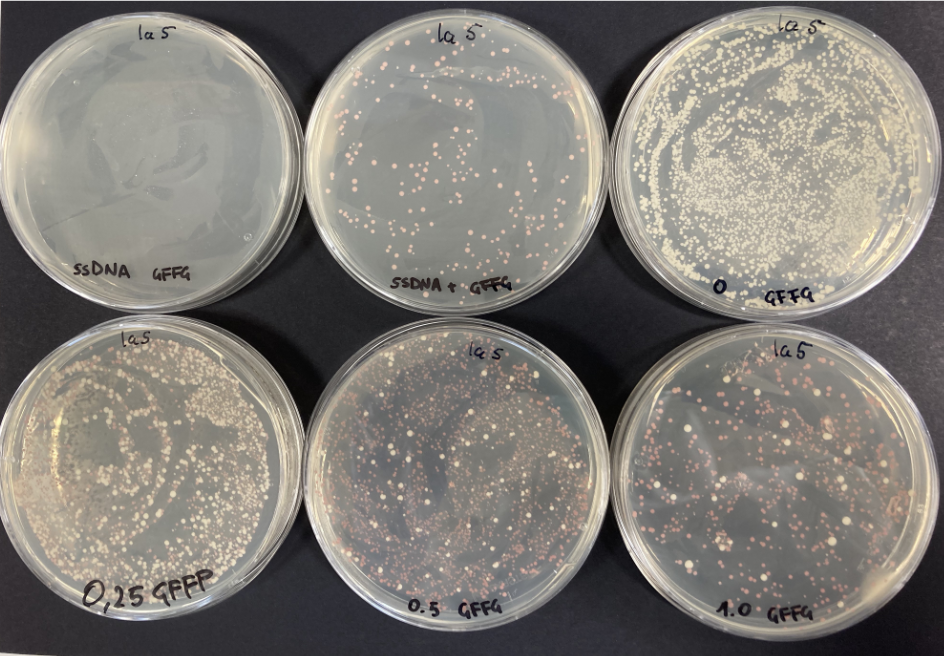
\includegraphics[scale=0.4]{./Pics/MutVitro/Contebatteriche.png}
		\caption{Colonie formatesi a diverse concentrazioni di \emph{$MnCl_2$}}
		\label{fig1}
	\end{figure}

	\begin{table}[H]
		\centering
		\begin{tabular}{|c|c|c|c|c|}
			\hline
			\makecell{Concentrazione di \emph{$MnCl_2$}} & $0M$ & $0.25M$ & $0.5M$ & $1M$\\
			\hline
			\makecell{Conta totale} & $2672CFU$ & $1822CFU$ & $1778CFU$ & $599CFU$ \\
			\hline
			\makecell{Colonie mutate} & $236CFU$ & $1044CFU$ & $1672CFU$ & $5564CFU$\\
			\hline
			\makecell{Tasso di mutazione} & $8.83\%$ & $57.3\%$ & $94\%$ & $94.16\%$\\
			\hline
		\end{tabular}
		\caption{Conta delle colonie}
		\label{tab}
	\end{table}

	\subsection*{Considerazioni finali}
	I risultati ottenuti, come si vede nella tabella~\ref{tab}, dimostrano come, non solo il cloruro di manganese riesca a competere con il magnesio per l'accesso al sito allosterico,
        ma anche quanto riesca a influire sia sull'efficienza della replicazione, che sulla sua precisione.
        Al crescere della concentrazione di manganese cloruro infatti, la conta totale di cellule in piastra, diminuisce, mentre aumenta la percentuale delle cellule mutate.
	Il tasso di mutazione nella coltura trasformata con il plasmide amplificato in assenza di manganese \`e imputabile all'affidabilit\`a della \emph{PCR}.
